\documentclass[output=paper]{langsci/langscibook} 
\ChapterDOI{10.5281/zenodo.3598562}



\title{Internal constituent variability and semantic transparency in N Prep N constructions in Romance languages} 

\author{Inga Hennecke\affiliation{University of Tübingen}}

% \chapterDOI{} %will be filled in at production

% \epigram{}

\abstract{Constructions of the type N Prep N represent one of the most controversial issues in Romance word formation. In particular, their lexical status and their degree of productivity are still crucial points of discussion. Hence, it remains unclear whether these constructions fall within the category of morphological word formation or of syntax. Furthermore, the possibilities for internal prepositional variation remain uncertain. This article takes a constructionist approach within the framework of construction morphology in order to describe the internal constituent variability and transparency of the prepositional element in N Prep N constructions in Spanish, Portuguese, and French, as in Sp. \textit{juego de niños}, \textit{juego para niños}  (`kid's game') or in Sp. \textit{cabaña de árbol} and \textit{cabaña en árbol} (`tree house'). A qualitative analysis of large-scale corpus data from the TenTen corpus family indicates that Romance N Prep N constructions may undergo internal prepositional variation. The analysis focuses on the semantic relations of the internal nominal constituents and the semantic transparency of the constructions in the three Romance languages under investigation. The results indicate that semantic relations and semantic transparency play a role in the internal constituent variability of the prepositional element.}

\shorttitlerunninghead{Internal constituent variability and semantic transparency}
\begin{document}

\maketitle
\section{Introduction} 
Compounds of the type N Prep N, such as Sp. \textit{bicicleta de montaña} `mountain bike', Fr. \textit{salle de bain} (`bath room'), or Pt. \textit{história em quadrinhos} (`comic strip'), are generally considered to be the most problematic aspect of research on compounding and word formation in Romance languages. This is because these constructions represent nominal lexical units that clearly approach free syntactic structures \citep{BustosGisbert:1986}. Compounds of the type N Prep N have been treated very differently in research on compounding and have also been labeled with many different terms, such as syntagmatic compounds \citep{BuenafuentesdelaMata:2010}, syntactic compounds \citep{RioTorto:2009}, improper compounds \citep{Kornfeld:2009}, phrasal lexemes \citep{Masini:2007}, frozen multiword units \citep{Guevara:2012}, lexicalized syntactic constructions \citep{Villoing:2012}, lexicalized phrases \citep{Fradin:2009}, and syntactic words \citep{DiSciullo:1987}. Generally, compounding is a mechanism whereby two lexical units are combined. Compounds of the type N Prep N are characterized as lexical units that consist of (at least) two lexical elements that are not orthographically combined. As a result, compounds of the type N Prep N, such as Sp. \textit{traje de baño} (`bathing suit'), do not differ on a formal level from syntactic phrases of the type N Prep N, such as Sp. \textit{libro para niños} (`book for children') \citep[69]{BustosGisbert:1986}.

The most problematic issue in current research on compounding of the type N Prep N is the question of the delimitation of syntactic and lexical structures in Romance languages. As the treatment of these constructions is based largely on the theoretical background of the individual author, there is no general agreement on whether or not N Prep N constructions should be included in the class of compounds. Related to this issue is the question of whether these constructions emerge by means of productive word formation processes or are merely ``fossilized'' or lexicalized syntactic structures. These two crucial issues will be discussed and analyzed in this study, with a focus on one particular case of internal constituent variability, the alternation of the internal preposition in N Prep N constructions. A large-scale corpus analysis of this alternation in French, Spanish, and Portuguese supports the adoption of a constructionist approach within a framework of construction morphology. Such an approach allows the internal constituent variation of N Prep N constructions to be represented without recourse to traditional notions of lexicon and syntax.


\section{Definition and classification of syntagmatic compounds} 

As mentioned above, constructions of the type N Prep N are often excluded from descriptions of Romance compounding.  Typically, they are classified together with other compound-like constructions lacking an orthographical union, as in the examples in \tabref{Fig:1:Types of phrasal lexemes}. 

\begin{table}
\caption{Phrasal lexemes in Romance languages \citep[257]{Masini:2009}\label{Fig:1:Types of phrasal lexemes}}
\begin{tabular}{lllll}
\lsptoprule 
Language & Types & Phrasal lexems & Lit. & Glosses\\ 
\midrule
French & [ADJ N]\textsubscript{N} & \textit{premier violon} & first violin & `first violin' \\  
Italian & [N \textit{da} N]\textsubscript{N} & \textit{camera da letto} & room from bed & `bedroom' \\  
Portuguese & [N \textit{de} N]\textsubscript{N} & \textit{cadeira de rodas} & chair of wheels & `wheelchair' \\  
Spanish & [N ADJ]\textsubscript{N} & \textit{luna nueva} & moon new & `new moon' \\ 
\lspbottomrule
\end{tabular} 
\end{table}

According to Masini, these examples are separated orthographically, show no strong degree of idiomaticity, and appear quite frequently in each of the four languages. The question nevertheless remains whether these constructions form part of the class of compounds.

According to \citet{Guevara:2012}, Spanish syntagmatic compounds, such as \textit{fin de semana} (`weekend') or \textit{sabelotodo} (`know-it-all'), should be excluded from the class of Spanish compounds, as these units are clearly syntactic units that contain “certain effects of lexicalization and atomicity in their distribution” \citep[180]{Guevara:2012}. In the same way, \citet{Villoing:2012} excludes French constructions such as \textit{fil de fer} (`iron wire') and \textit{brosse à dents} (`tooth brush') from her description of French compounds, as they are “lexicalized syntactic constructions that behave like lexical units” \citep[35]{Villoing:2012}. The approach taken by Guevara and Villoing indicates, on the one hand, that constructions of the type N Prep N are often considered as syntactic units that lie outside of the core of word formation processes. For this reason, they are regularly neglected in research papers on Romance word formation. On the other hand, this approach shows that N Prep N constructions are frequently interpreted as lexicalized syntactic constructions and, more precisely, as syntactic constructions that have somehow attained a high degree of fixedness. If this is the case, they should also be excluded as belonging to the class of Romance-language compounds, as lexicalization cannot be considered a morphological word formation process.

There is an opposing perspective according to which the constructions mentioned in \tabref{Fig:1:Types of phrasal lexemes} constitute a productive type of word formation and clearly follow productive morphosyntactic rules. According to Rainer, constructions of the type N Prep N are “very productive lexical patterns, which normally continue to obey the rules of […] syntax (for example, agreement rules), but may occasionally also deviate from them” \citep[2724]{Rainer:2016}. This perspective is not new and was already adopted by \citet{Benveniste:1974} in his work on French compounds of the type \textit {robe de chambre} (`robe') and \textit {plat à barbe} (`shaving bowl'), for which he claims indefinite productivity \citep[172]{Benveniste:1974}. In the course of the present paper, I will provide new empirical evidence in favor of this perspective using large-scale corpus data. The analysis will show that N Prep N constructions in Romance languages are highly frequent and productive and that their internal variability follows clear morphological rules that can be mapped using construction morphology.

In order to distinguish N Prep N constructions from other phrase-like constructions, their characteristics must be clearly delineated. According to \citet{BuenafuentesdelaMata:2010}, a syntagmatic compound may be defined as a lexical element that has been created by the fixation of a syntagm, which keeps its sentential structure, and therefore shows neither orthographic nor accentual union \citep[21ff.]{BuenafuentesdelaMata:2010}. \Citet{BustosGisbert:1986} states that Spanish N Prep N compounds differ from syntactic units on the syntactic level in two respects. First, they have a fixed word order, for example, \textit{ojo de buey} (`porthole') cannot be reordered as *\textit {buey ojo de}. Second, there is generally no unproblematic substitution of their constituents; for example *\textit{ojo de vaca} (`eye of cow') \citep[4825]{ValAlvaro:1999}. On a morphological level, he adds that N Prep N constructions show the same characteristics as other compounds in terms of gender and number agreement, the presence of composition markers, and the ability to undergo further derivation and to form collocations \citep[77]{BustosGisbert:1986}. According to Masini, N Prep N constructions are of major interest, as they follow the syntactic rules of head modification of a nominal phrase by a prepositional phrase. This means that in Romance languages, N Prep N constructions are generally left-headed, and that inflectional processes are performed on the head of the construction \citep[257]{Masini:2009}. \citet[4827]{ValAlvaro:1999} adds a fundamental characteristic on the semantic level: the absence of compositional meaning that may lead to syntactic reinterpretation of the complex nouns. This means that syntagmatic compounds, in contrast to syntactic units, represent one single naming unit at the semantic level; that is, they refer to one specific conceptual representation, as in Fr. \textit{sac à main} (`purse').

In this paper, I will focus on the syntactic criteria given by de Bustos Gisbert, specifically, on the impossibility of constituent substitution. This criterion does not appear to be suitable for purposes of differentiating syntactic and lexical elements, as the delimitation between syntactic and lexical N Prep N constructions remains a matter of controversy. Here, I will show that variation of the internal preposition can be best explained within a constructional framework. I will then argue with regard to the internal preposition that not only is the substitution of internal constituents possible in N Prep N constructions, but it is also a rule-governed process and depends largely on semantic factors, particularly the semantic relation of the nominal constituents.

When investigating the semantic relations of constituents of N Prep N constructions, it is crucial to consider the notions of semantic transparency and semantic opacity. In current research, the term semantic transparency refers to the degree to which the meaning of a complex construction can be derived from the meaning of its constituents \citep{Zwitserlood:1994}. For example, the French N Prep N construction \textit{salle de bains} (`bathroom') is considered semantically transparent, whereas the Spanish construction \textit{ojo de buey} (`porthole', lit. `bull's eye') is considered semantically opaque. Bell and Schäfer view semantic transparency and semantic opacity as scalar notions, lying at either end of a continuum (see \citet{Bell:2016} for a detailed discussion on semantic transparency). Later in the present study, I will discuss whether the semantic transparency of an N Prep N construction determines the possibility of internal constituent variation.

\section{Internal constituent variation in N Prep N constructions: The role of the preposition} 
Characteristic of N Prep N constructions, and a crucial factor in their delimitation, is their resistance to paradigmatic variation. In the context of the delimitation of nominal compounds and noun phrases of the type N Prep N in Portuguese, \citet[9]{RioTorto:2012} state that the ``(im)possibility of lexical insertion" is one of the most important tests of compoundhood. They go further, claiming that if internal changing is allowed, ``we are no longer dealing with compounds ([N[PrepN]]\textsubscript{N})  but with noun phrases ([N[PrepN]]\textsubscript{NP})" (ibid.). When speaking of internal change, Rio-Torto and Ribeiro refer principally to changes in determination, as in Pt. \textit{fim de semana} (`weekend') and Pt. \textit{fim da semana} (`end of this week'), and to changes effected through insertion of lexical material, as in \textit{fim da última semana} (`end of last week'). As these examples suggest, internal constituent variation is generally seen as a crucial test of delimitation between compounds and syntactic structures. Similarly, Masini argues that, for lexical elements, ``paradigmatic variation is blocked, since the words in the construction cannot be substituted by a near-synonym, which should not be a problem for normal phrases" \citep[259]{Masini:2009}. Masini defines paradigmatic blocking as the inability to replace a constituent of the construction by another paradigmatically fitting constituent. She also refers to cases of paradigmatic blocking of a nominal unit of a N Prep N construction, as the Italian examples \textit{casa di cura} (`nursing home') and *\textit{abitazione di cura} (`*nursing domicile'). In this case, \textit{casa di cura} is a fixed naming unit that loses its semantic meaning when there is paradigmatic variation of a nominal element. The following analysis will show that paradigmatic blocking holds particularly true for N Prep N constructions with a stronger degree of semantic opacity and idiomaticity. More transparent N Prep N constructions allow productive and rule-governed internal constituent alternation, as the analysis will show by means of the prepositional constituent.
 
In the literature, all references to a delimitation test of constituent variability neglect the prepositional constituent in N Prep N constructions. The prepositional element is fundamental in N Prep N constructions, but its status is far from clear. In all the Romance languages under investigation here, the preposition \textit{de} is the most frequently used prepositional constituent in N Prep N constructions. In the case of Spanish, \citet{BuenafuentesdelaMata:2010} cites various examples of N Prep N constructions with prepositions other than \textit{de}, such as \textit{leche en polvo} (`milk powder'), \textit{cita a ciegas} (`blind date'), \textit{caridad con uñas} (`self-serving favor'), \textit{pozo sin fondo} (`bottomless pit'), and \textit{caballo con arcos} (`pommel horse'). She adduces the appearance of prepositions other than \textit{de} as evidence for the structural complexity of N Prep N constructions in Spanish. The same case can be made for the other languages under investigation in this paper (i.e. French and Portuguese), which show the same ability to form N Prep N constructions with other prepositions.
 
 This paper concentrates on a specific set of (partially) synonymous prepositions in French, Spanish, and Portuguese, which are Fr. \textit{de} (`of'), \textit{à} (`to'), \textit{en} (`in'), and \textit{pour} `for'; Sp. \textit{de} (`of'), \textit{a} (`to'), \textit {en} (`in'), and \textit{para} (`for') as well as Pt. \textit{de} (`of'), \textit{a} (`to'), \textit{em} (`in') and \textit{para} (`for'). These prepositions may all appear in N Prep N constructions and they may all undergo internal alternation and variation in the three languages under investigation. Consider examples \xxref{ex:hennecke:1}{ex:hennecke:3} from the TenTen corpora:
 
\ea \label{ex:hennecke:1}
  \ea\label{ex:hennecke:1a} Sp. \textit{fuente de horno – fuente para horno}   `casserole' \\ 
  \ex\label{ex:hennecke:1b} Pt. \textit{água de lavagem – água para lavagem}     `wash water' \\ 
  \ex\label{ex:hennecke:1c} Fr. \textit{livre d'enfant – livre pour enfants}    `children’s book' \\ 
 \z
\ex  \label{ex:hennecke:2}
  \ea\label{ex:hennecke:2a} Sp. \textit{motores de gasolina – motores a gasolina}    `gas engine' \\ 
  \ex\label{ex:hennecke:2b} Fr. \textit{jauge d'essence – jauge à essence}   `fuel gauge' \\ 
  \ex\label{ex:hennecke:2c} Pt. \textit{fogão de lenha – fogão a lenha}   `wood stove' \\ 
 \z
\ex \label{ex:hennecke:3}
  \ea\label{ex:hennecke:3a} Fr. \textit{chemise de coton – chemise en coton}   `cotton shirt' \\ 
  \ex\label{ex:hennecke:3b} Pt. \textit{bracelete de aço – bracelete em aço}  `steel bracelet' \\ 
  \ex\label{ex:hennecke:3c} Sp. \textit{ciclismo de pisto – ciclismo en pisto}   `track cycling' \\ 
  \z
\z
 
Example \REF{ex:hennecke:1} shows internal variation of the prepositional elements \textit{de} and \textit{pour/para}. While the constructions containing \textit{de} are considered to have a lexical status, the constructions with \textit{pour/para} are generally considered to be syntactic constructions, as they pass certain of the classification tests mentioned above. In contrast to the construction with \textit{de}, they allow substitution and insertion, as the two tests of compoundhood demonstrate: Sp. \textit{fuentes de vidrio para horno} (`glass casseroles for the oven'), \textit{fuentes profundas para horno} (`deep casseroles for the oven'), but *\textit{fuentes de vidrio de horno} and *\textit{fuentes profundas de horno}. Example \REF{ex:hennecke:3b} demonstrates the internal alternation of the prepositions \textit{de} and \textit{en/em}. Here, alternation is possible without changing the semantic context of the whole construction or its degree of semantic transparency. In example \REF{ex:hennecke:2}, the prepositions \textit{de} and \textit{a/à} alternate in N Prep N constructions without changing the lexical status of the respective constructions. Nonetheless, these constructions differ in their frequency of usage, productivity, and fixedness, as well as in their degree of lexicalization and of idiomaticity. Especially in French, alternation of \textit{de} and \textit{à} may indicate a change in meaning, as in \textit{verre de vin} (`glass of wine') and \textit{verre à vin} (`wine glass'). In this case, the interpretation of both constructions as two distinct products of word formation is reasonable (this specific case will be discussed in detail in the course of the corpus analysis). In other cases, such as Pt. \textit{fogão de lenha – fogão a lenha} (`wood stove'), no clear semantic difference is visible, as attested by native speakers of Brazilian and European Portuguese: internal variation is possible inside one construction (a more detailed discussion of the examples will follow in the upcoming section). As mentioned above, authors including \citet{RioTorto:2009} interpret constructions of the type shown in examples \xxref{ex:hennecke:1}{ex:hennecke:3} as syntactic units, on the grounds that they do not pass all the delimitation tests for compoundhood. The following theoretical discussion and empirical analysis will show that it is neither necessary nor possible to draw a clear distinction between syntactic constructions and lexical constructions; the possibility of alternating prepositional elements in N Prep N constructions depends largely on the semantic function of the N2, and the fixedness, semantic transparency and the idiomaticity of the whole construction.
  
Another problem in analyzing alternation of prepositional elements concerns the role of the prepositions. In Romance languages, the prepositions \textit{de} and \textit{à/a} in particular have often been considered as semantically ``empty'' units that do not contain meaning. This perspective has often been applied to the prepositional element in N Prep N constructions: for example, \citet[164]{Bartning:1993} states that prepositions in French N Prep N constructions do not code any specific meaning and that they function only as linking elements. Similarly, \citet{Bartning:1993} refers to \citet{Cadiot:1997} by describing these prepositional elements as ``colorless prepositions'' \citep[164]{Bartning:1993}. For the French prepositions \textit{de} and \textit{à}, \citet[44]{Bosredon:1991} use the term of ``opérateur de couplage" (`linking operator'). \citet{Cadiot:1997} sees prepositions in N Prep N constructions as elements that express the operation of a construction or the denomination of a subclass of N1; he associates the prepositional element with a ``referential calibration'' of N1. In contrast, \citet[32]{Laumann:1998} notes the importance of distinguishing between different types of meaning when investigating the function and meaning of prepositions in nominal compounds. He differentiates between system meaning (\textit{Systembedeutung} -- the sum of the meaning patterns of the constituents in the N Prep N construction), word meaning (\textit{Wortbedeutung} -- the meaning of the construction on the level of word formation), and lexicon meaning (\textit{Wortschatzbedeutung} - the meaning of the construction as a naming unit in the lexicon).

Other authors interpret the possibility of elision of the prepositional element, as Sp. \textit{ducha de teléfono}  > \textit{ducha teléfono} (`detachable shower head') or Sp.  \textit{crédito de vivienda} > \textit{crédito  vivienda} (`home loan'), as evidence of the semantic emptiness of the preposition. However, the elision of the prepositional element is only possible in certain strongly lexicalized constructions. Therefore, a counterargument may be based on the same evidence, given that the elision of the prepositional element is not possible in most cases. In the present paper, I argue that the elision of prepositional elements is not proof of a lack of semantic content. The elision can be explained in terms of common processes of language change that may or may not take place in certain lexicalization processes within complex units. The alternation between prepositional elements, as exemplified above is a productive word-formation process that differs clearly from mere lexicalization processes. Therefore, the following qualitative corpus analysis considers the internal constituent alternation of the prepositional element from a comparative perspective and does not focus on the elision of this element. The analysis adopts a constructionist approach based on \citet{Goldberg:1995,Goldberg:2006}, with a special focus on construction morphology as introduced by \citet{Booij:2010,Booij:2015}.

\section{N Prep N constructions in construction grammar and morphology}\label{sec:henneke:4}
Since Goldberg’s seminal work \textit{Constructions} (\citeyear{Goldberg:1995}), the constructional approach has had a strong impact on linguistic research. Constructions are considered as conventionalized form-meaning pairs that can be found at all levels of abstraction in language, are dynamically formed, and may be changed continuously. They are acquired via general processes of abstraction, generalization, and categorization. \citet[5]{Goldberg:2006} considers any linguistic unit to be a construction, if ``some aspect of its form or function is not strictly predictable from its component parts''. Furthermore, units are considered to be stored as constructions if they can be fully predicted and if they are sufficiently frequent (ibid.).

In his theory of construction morphology, \citet{Booij:2015} applied the general notions and concepts of construction grammar to morphological units that have traditionally been regarded as morphological. The underlying assumption of the theory of construction morphology is that a construction may have characteristics that cannot be derived from their constituents \citep[3]{Booij:2015}. Booij cites the example of the reduplication of nouns in Spanish in order to express the notion `real', as in \textit{un café café} (`a real coffee'). He establishes the notion of conceptual schemas and subschemas, defined as schematic representations of morphological constructions. These schemas represent a correlation between form and meaning:

\ea\citep[2]{Booij:2015}\\ <[[x]V\textsubscript{i} er]N\textsubscript{j} $\leftrightarrow$ [Agent of SEM\textsubscript{i}]\textsubscript{j}>\z

This example indicates that a word with base x, in this case an English infinitive verb form, can transform into a noun with the meaning `agent of the base word (SEM)' by adding the suffix \textit{-er} \citep[2]{Booij:2015}. The variable x denotes the phonological content of the base word, i denotes the meaning of the base word, and j shows that the meaning of the complete construction depends on the form of the complete construction (ibid.). \citet[261]{Masini:2009} applies the theory of construction morphology to constructions of the type N Prep N in Italian, taking them to represent an abstract template that is stored in the mental lexicon. Masini further notes that this abstract template features a certain degree of productivity and is associated with a concrete naming function (ibid.). By means of a specific inheritance mechanism, based on instance inheritance links \citep{Goldberg:1995}, constructions that are more and more specific can be derived from the abstract template. This may be done by categorical specification (filling an unspecified slot with a specific category), as in N Prep N or N Prep V, by lexical specification (filling a slot with specific lexical material), as in N \textit{de} N or by a completely lexical construction, such as It. \textit{casa di cura} \citep[261]{Masini:2009}. \figref{fig:hen:1} demonstrates the application of this theory to French constructions of the type N Prep N.

\begin{figure}
\caption{Inheritance hierarchy for N Prep N templates in French \citep[263]{Masini:2009}\label{fig:hen:1}}
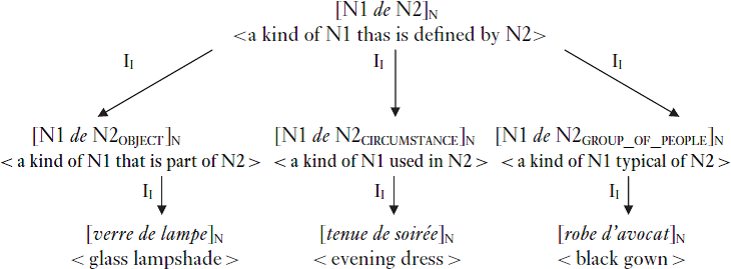
\includegraphics[scale=0.5]{figures/Masinifigure2.png} 
\end{figure}

This figure shows the inheritance hierarchy from the abstract template [N1 \textit{de} N2]\textsubscript{N}, which here is an intermediate construction of the abstract template [N1 Prep Y] and [N1 Prep N2]. From the level [N1 \textit{de} N2]\textsubscript{N}, it is possible to proceed to a second intermediate lexical level, which indicates the semantic function of N2, and to conclude at a completely lexical level, which shows the lexical result with a concrete naming function. According to \citet[263]{Masini:2009}, this model can also clarify and describe new occurrences of the N1 \textit{de} N2 construction. 

The following qualitative corpus analysis aims to apply the concept of construction morphology presented by \citet{Booij:2010,Booij:2015} and exemplified by \citet{Masini:2009} to a cross-linguistic comparative analysis of large-scale corpus data for Spanish, French, and Portuguese N Prep N constructions. The focus of the analysis is on constituent variation of the internal prepositional element in N Prep N constructions in these three languages, and I will apply Masini's inheritance hierarchy template (\figref{fig:hen:1}) to the internal variability of prepositional constituents. It is useful to include a further intermediate level prior to the first and second levels of the hierarchy for N Prep N templates mentioned above. This additional level contains the abstract template with the semantic function of N2, which in the following corpus analysis is shown to be a crucial factor in determining the possibility of internal prepositional variation. For the purposes of the present analysis, the inheritance hierarchy for N Prep N templates may be visualized as in \figref{fig:henneke:Inheritancehierarchy}.

\begin{figure}
\caption{Inheritance hierarchy for internal variation in N Prep N templates in French (adapted from \citealt{Masini:2009})\label{fig:henneke:Inheritancehierarchy}}
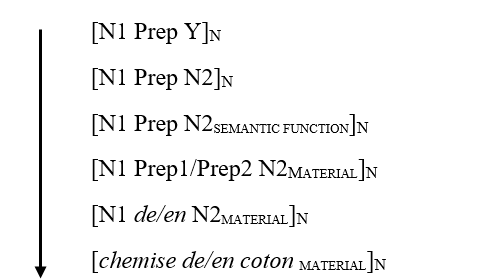
\includegraphics[scale=0.5]{figures/Inheritancehierarchy.png} 
\end{figure}

This figure shows the inheritance hierarchy adapted from \figref{fig:hen:1} by means of example \REF{ex:hennecke:3a}. As mentioned above, the added abstract intermediate levels are intended to reflect the possibility of that prepositional variability for certain N Prep N constructions and the dependence of this variability on the semantic function of the nominal constituents of the construction. The objectives of the following qualitative corpus analysis are to apply the inheritance hierarchy in \figref{fig:henneke:Inheritancehierarchy} to a large-scale corpus of natural speech data for Spanish, French and Portuguese and to compare the internal prepositional variability of N Prep N constructions in these three languages.

\section{Qualitative corpus analysis}
 As mentioned above, the present corpus analysis is intended to investigate internal constituent alternation of the prepositional element in N Prep N constructions in Spanish, French and Portuguese. The focus is on the alternation between \textit{de} and \textit{à/a}, \textit{de} and \textit{en/em}, and \textit{de} and \textit{pour/para}. This study builds on a quantitative corpus survey on the internal alternation of the prepositional element in N Prep N constructions in Spanish, French, and Portuguese by means of large-scale corpus data \citep{Hennecke:2017}. \citet[144]{Hennecke:2017} showed that internal prepositional variation in the three languages under investigation is possible, but that these languages show different characteristics in terms of frequency and productivity of such alternations. The quantitative analysis of the three languages focused on frequency of types and token, productivity (i.e. probability of previously unobserved types), and population size (i.e. potential number of formations) \citep[139]{Hennecke:2017}. The results show that Portuguese and, to a lesser extent, French, allows productive internal constituent variation of the prepositional element. In contrast, Spanish does not show productivity in internal variation, which is demonstrated by the absence of hapax legomena (ibid.). At the same time, Spanish has the greatest tendency to employ the preposition \textit{de} in N Prep N constructions. In French, the prepositions \textit{à} and \textit{pour} are slightly more productive than in the other two languages. Moreover, French tends to avoid constructions using \textit{avec}, whereas constructions with \textit{com} are productive in Portuguese. The latter tendency may be explained by the fact that French prefers NA-constructions over constructions of the type N \textit{avec} N.
 
The aim of the present corpus analysis is to investigate the results from the above-mentioned study from a qualitative perspective. In this qualitative survey, the internal prepositional variability will be investigated from a mostly semantic perspective, combined with a constructionist approach. Here, the focus will be on which nominal semantic functions allow prepositional variability and whether the variability depends on the semantic transparency of the construction. To that end, this corpus analysis is based on the same dataset as in \citet{Hennecke:2017}, namely three web corpora from the TenTen corpus family from Sketchengine: the French corpus frTenTen12, the Spanish corpus esTenTen11 and the Portuguese corpus ptTenTen11. The TenTen corpora are large-scale web corpora with the counts displayed in \tabref{tab:1:frequencies}.

\begin{table}
\caption{Corpus Information of the TenTen corpora for Spanish, French and Portuguese (\url{https://the.sketchengine.co.uk})\label{tab:1:frequencies}}
 \begin{tabular}{lrrr} 
  \lsptoprule
            & frTenTen12 & esTenTen11 & ptTenTen11 \\ 
  \midrule
  Tokens  &   11,444,973,582 &    10,994,616,207     & 4,626,584,246\\
  Words  &   9,889,689,889 &  9,497,402,122 &    3,900,501,097\\
  Sentences  &  456,065,104 &  407,205,587 &    190,221,913\\
  Paragraphs  &  188,079,362 &  213,364,685 &    91,248,976\\
   Documents  &  20,400,411 &  22,287,566 &    10,216,060\\
  \lspbottomrule
 \end{tabular}
\end{table}


In order to perform a qualitative analysis of the data, all N Prep N constructions were extracted automatically from the corpora, keeping only those that appear with more than one internal prepositional element. The present analysis focuses exclusively on N Prep N constructions and therefore excludes constructions of the type N Prep Det N. The data were manually inspected by excluding grammaticalized constructions (for example Fr. \textit{face à N}, Sp. \textit{gracias a N} `thanks to N'), binominal pairs (e.g. Fr. \textit{temps en temps} `time to time', Sp. \textit{dia a dia} `day to day'), and antonyms (Fr. \textit{chien avec/sans laisse} `dog with/without leash'). \tabref{tab:2:frequencies} demonstrates the underlying dataset for the qualitative analysis.

\begin{table}
\caption{Type and token counts for the underlying dataset with all pairs of nouns that are attested with at least two different internal prepositions\label{tab:2:frequencies}}
 \begin{tabular}{lrr} 
  \lsptoprule
            & Types & Tokens \\ 
  \midrule
  French  &   1062 &    6991     \\
  Spanish  &  547 &  10219 \\
  Portuguese  &  6795 &  58932 \\
  \lspbottomrule
 \end{tabular}
\end{table}

This dataset shows important differences in type-token frequency between the three languages \citep{Hennecke:2017}. Portuguese presents by far the greatest number of different types and tokens of N Prep N constructions with more than one internal preposition. In contrast, Spanish has very few different types but a considerable number of tokens. This can be interpreted as a small number of different N Prep N constructions, but these few types appear quite often in the corpus data. The French data show a significantly higher number of different types than the Spanish data, but a lower number of different tokens. Here, more different types occur less often in the corpus data (for a detailed quantitative analysis of the data see \citealt{Hennecke:2017}). In what follows, a qualitative analysis of selected pairs of internal prepositions is presented in order to investigate whether these differences also appear at a qualitative level, with a special focus on the semantic functions of the nominal constituents and the semantic transparency of the constructions. The specific semantic relations were established with regard to the current literature on the semantic relations of nominal constituents in nominal compounds \citep{Gagne:1997, Gagne:2009, Girju:2005}. They were subsequently modified and adapted to the specific case of N Prep N constructions in the corpus data under investigation. It is not possible to list and discuss all occurrences of all types in the present paper; only selected examples will therefore be discussed and analyzed. Where necessary, references will be made to frequency of occurrence. 

\subsection{The preposition \textit{de} in N Prep N constructions}
In all three languages under investigation, the preposition \textit{de} is most often used to combine two nominal expressions, as in Fr. \textit{salle de bain}  (`bathroom'), Sp. \textit{botas de agua} (`rubber boots'), or Pt. \textit{moinho de vento} (`wind mill'). Therefore, the preposition \textit{de} appears in all pairs of internal prepositional variation analyzed in the following section. The three data sets also show internal variation for prepositions other than \textit{de}, but these pairs are not the subject of the present analysis. As mentioned above, the preposition \textit{de} has been much discussed; it has often been considered an ``empty'' or ``colorless'' preposition that lacks any kind of semantic content and that merely fulfills a linker role functions. This completely functional approach is not adopted in the present paper for reasons given above.
In the present account, I follow a constructionist approach (see \citealt{Masini:2009}), in which the prepositional constituent in N Prep N constructions is an element of semantic consequence to the whole construction \citep[262]{Masini:2009}. Masini states the example of Italian N1 \textit{di} N2 intermediate lexical constructions, which clearly differ semantically from N1 \textit{a} N2 intermediate lexical constructions. With reference to Johnston and Busta (1996), she emphasizes that  ``the prepositions \textit{da}, \textit{di} and \textit{a} in Italian N+PREP+N expressions, under certain conditions and in combination with certain classes of nouns, are specialized for different kinds of modification" \citep[262]{Masini:2009}. In the further analysis, the statement from Masini will be refined, since in the present data, the intermediate lexical constructions N1 \textit{de} N2 and other intermediate lexical constructions (e.g. \textit{N1 para/pour} N2) may overlap semantically under certain conditions. These cases will be exemplified below in a cross-linguistic comparative analysis. In this analysis, the preposition is seen not as a semantically opaque constituent but as a constituent with a specific semantic value determined by the semantic functions of the nominal constituents.

The preposition \textit{de} in French, Spanish, and Portuguese has been described as expressing various relations \citep[187]{Bartning:1993}. In binominal constructions, it expresses, for instance, a relation of possession (Sp. \textit{el ordenador de Luis} `Luis' computer', Fr. \textit{la voiture de Jean} `John’s car'), characterization (Fr. \textit{statut de valeur} `status'), instrument (Fr. \textit{coup de baton} `blow'), material (Fr. \textit{papier de soie} `silk paper'), a part-whole relation (Sp. \textit{puerta de casa} `front door', Pt. \textit{ponta do dedo} `fingertip'), an affiliation (Fr. \textit{fils de roi} `king’s son'), a content (Fr. \textit{tasse de café} `cup of coffee'), a defining characteristic (Sp. \textit{hotel de lujo} `luxury hotel') or a purpose (Pt. \textit{vestido de noiva} `wedding dress'). For more examples in French see \citet[291ff.]{Lang:1991}.

\subsection{Internal variation between \textit{de} and \textit{a/à}}

Internal variation between the prepositional constituents \textit{de} and \textit{à} has been the subject of several articles and books on French prepositions and nominal syntagms (e.g. \citealt{Anscombre:1990, Lang:1991, Bosredon:1991, Cadiot:1997}). However, it is interesting that this discussion has no equivalent in the literature on Spanish and Portuguese prepositions. This is because such internal variation does not take place in Spanish and only to a small extent in Portuguese. The sole example of internal variation of \textit{de} and \textit{a} in the Spanish corpus data is the following:

\ea\relax [N1 \textit{de/a} N2\textsubscript{\scshape type/specification}]\textsubscript{N}>		\textit{freno de/a disco},	`disk brake'\z

Here, the construction containing \textit{de} is far more frequent and the lexicalized form can be found in dictionaries. Still, the construction \textit{freno a disco} also occurs regularly in the corpus data of the esTenTen corpus, with a frequency of 0.10 occurrences per million. However, the corpus data shows that the internal variation of \textit{de} and \textit{a} is neither frequent nor productive in Spanish, as only one example of one type can be found in this large-scale internet corpus. In Portuguese, the ptTenTen data shows at least two Intermediate lexical constructions with variation of \textit{de} and \textit{a} that present a certain productivity:

\begin{exe}\ex\begin{minipage}[t]{0.4\textwidth}    %an der Zahl 0.4 kannst du herumspielen für die Breite
[N1 \textit{de/a} N2\textsubscript{\scshape purpose}]\textsubscript{N}\\
\textit{forno de/a microondas,  forno de/a lenhas}\\
`microwave oven',         `wood stove'
\end{minipage}\hfill    %für den Abstand zwischen den Spalten, Leerzeilen funktionieren nicht
\begin{minipage}[t]{0.45\textwidth}
[N1 \textit{de/a} N2\textsubscript{\scshape type/specification}]\textsubscript{N}\\
\textit{lampião de/a gás,   pilhas de/a combustível }\\
`gas lantern',           `fuel cell'
\end{minipage}%
\end{exe}

\hspace*{-1.11124pt}The template [N1 \textit{de/a} N2\textsubscript{\scshape type/specification}]\textsubscript{N}, in particular, is frequently present in the corpus data and is expressed via different types, as in \textit{motor de/a combustão} (`combustion motor') or \textit{bomba de/a vácuo} (`vacuum pump'). It is striking that many of these types are technical terms. It is possible to perceive a semantic difference in both intermediate constructions, where the type N1 \textit{a} N2 more clearly indicates the material part of the N2 constituent, the type N1 \textit{de} N2 focuses semantically on complementing N1 and creating a construction that is a subtype of N1. However, the first sample surveys and questionnaires revealed that native speakers of European and Brazilian Portuguese do not perceive a difference in the semantic meaning patterns or, more precisely, in the semantics of the whole construction.

For the French data, a very different pattern appears in the analysis of internal variability of \textit{de} and \textit{à}:

\begin{exe}\ex\begin{minipage}[t]{0.4\textwidth}    %an der Zahl 0.4 kannst du herumspielen für die Breite
[N1 \textit{de/à} N2\textsubscript{\scshape purpose}]\textsubscript{N}\\
\textit{fil de/à pêche}\\
`fishing rod'
\end{minipage}\hfill            %für den Abstand zwischen den Spalten, Leerzeilen funktionieren nicht
\begin{minipage}[t]{0.45\textwidth}
[N1 \textit{de/à} N2\textsubscript{\scshape type/specification}]\textsubscript{N}\\
\textit{course à/d’obstacles}\\
`obstacle course'
\end{minipage}%
\end{exe}

\begin{exe}\ex\begin{minipage}[t]{0.4\textwidth}
[N1 \textit{de/à} N2\textsubscript{\scshape ingredient}]\textsubscript{N}\\
\textit{crème au/de citron}\\
`lemon creme'
\end{minipage}\hfill\begin{minipage}[t]{0.45\textwidth}
[N1 \textit{de/à} N2\textsubscript{\scshape container}]\textsubscript{N}\\
\textit{conteneur de/à déchets }\\
`waste bin\slash bin with waste'
\end{minipage}%
\end{exe}

\ea\relax
[N1 \textit{de/à} N2\textsubscript{\scshape transport}]\textsubscript{N}\\
\textit{course de/à vélo}\\
`biking trip'
\z

The existing literature on \textit{de-à} alternation in French emphasizes that there is a semantic difference between binominal constructions containing \textit{de} and \textit{à} and that this semantic difference affects not only the prepositional element itself but also the whole naming unit. This becomes very clear in more detailed analysis of the examples from the template [N1 \textit{de/à} N2\textsubscript{\scshape container}]\textsubscript{N}. In all these examples, the intermediate lexical construction N1 \textit{à} N2 designates the container itself, as in \textit{flûte à champagne} (`champagne glass') or \textit{corbeille à fruit} (`fruit bowl'). In contrast, the intermediate lexical construction N1 \textit{de} N2 denotes the content of the container, as in \textit{flûte de champagne} (`a glass of champagne') or \textit{corbeille de fruit} (`a bowl of fruits'). In these cases, according to \citet{Cadiot:1997}, \textit{de} turns the interpretation of the construction toward the N2 and constructs a quantified image of the referent, whereas \textit{à} turns the interpretation toward the N1 and permits a qualified image of the reference \citep[44]{Cadiot:1997}. That is, \textit{de} carries an effect of quantification whereas \textit{à} carries a semantic notion of qualification. For cases of the intermediate lexical construction [N1 \textit{de/à} N2\textsubscript{\scshape ingredient}]\textsubscript{N}, such as \textit{salade d’écrevisses} and \textit{salade aux écrevisses} (`crawfish salad'), \citet{Lang:1991} states that the preposition \textit{à} connects N1 and N2, whereas the preposition \textit{de} derives N1 from N2. That is to say that \textit{à} describes an ingredient, whereas \textit{de} describes a substance \citep[283]{Lang:1991}. In the same way, in the examples of [N1 \textit{de/à} N2\textsubscript{\scshape type/specification}]\textsubscript{N} and [N1 \textit{de/à} N2\textsubscript{\scshape means of transport}]\textsubscript{N}, it can be seen that \textit{à} points to the material object \textit{vélo} or \textit{obstacles}, whereas  \textit{de} more likely complements the N1, and hence the whole construction describes a subtype of N1. According to \citet[43]{Cadiot:1997}, the semantic differences that occur through the variation of the prepositions \textit{de} and \textit{à} can be accounted for in terms of the more abstract categorization that is the opposition of intension and extension. On this view, \textit{de} constructs an extensional reference  directly, whereas \textit{à} creates an extensional reference  indirectly by passing over an intentional reference \citep[62]{Cadiot:1997}. 

From a constructionist perspective, it can be stated that only in the template [N1 \textit{de/à} N2\textsubscript{\scshape container}]\textsubscript{N} does the semantic value of the whole construction\linebreak change, as in \textit{conteneur de déchets} (`bin containing waste') and \textit{conteneur à déchets} (`waste bin'). In this case only, we have two different naming units when \textit{de} and \textit{à} alternate. Therefore, only here is it appropriate to refer to two different constructions, [N1 \textit{de} N2\textsubscript{\scshape container}]\textsubscript{N} and  [N1 \textit{à} N2\textsubscript{\scshape container}]\textsubscript{N}, which lead to two different naming units at the lexical level. In all the other cases mentioned above, the variability of \textit{de} and \textit{à} does not lead to different semantic interpretations of the lexical outcome, but only to a difference in the semantic weight of certain meaning patterns in the interpretation. Therefore, in all other cases, the inheritance hierarchy from the previous section of this paper can be applied in order to capture the internal constituent variation.

To conclude this analysis, it can be stated that all constructions that allow internal constituent variation of the prepositional element are semantically transparent.  The analysis shows that alternation of the internal prepositional constituent does not go along with the semantically more opaque constructions in the languages under investigation, since normally in these cases, the semantic functions of the nominal constituents cannot always be clearly determined. In Spanish and Portuguese, the internal variation is only possible in very specific cases of semantic function of the nominal constituents. In French, on the other hand, the internal variation of \textit{de} and \textit{à} is more frequently used or observed, and appears to be governed by the semantic functions of the nominal constituents.

\subsection{Internal variation between \textit{de} and \textit{em/en}}

The variation between \textit{de} and \textit{en/em} in N Prep N constructions has received little attention in the literature. On a general level, \citet[411]{Lang:1991} states that in French, \textit{en} between two nouns indicate the location of N1, as in \textit{arc-en-ciel} (`rainbow') and \textit{une ville en Italie} (`a city in Italy'), the characterization of N1, as in \textit{ange en stuc} (`stucco angel'), a way of preparation of N1, as in \textit{une salade en vinaigrette} (`a salad with dressing'), the material of N1, as in \textit{robe en soie} (`silk dress'), the form in which N1 appears, as in \textit{fleurs en bouquet} (`bouquet of flowers'), the condition in which N1 stands, as in \textit{arbre en fleur} (`blooming tree'), or a field in which N1 operates, as in \textit{expert en assurances} (`insurance expert'). According to \citet[55]{Laumann:1998}, French \textit{de} and \textit{en} are not always interchangeable when N2 refers to the material of N1. On the basis of an analysis of French grammar and dictionary entries, Laumann states that \textit{en} appears more regularly with a predicative supplement than \textit{de}, gives more concrete information about the material, and is less strongly linked to the N1. However, the most important difference seems to be that \textit{en} cannot appear in more opaque constructions with a (partially) idiomatic reading. \citet[55]{Laumann:1998} cites the examples of \textit{homme de fer} (`iron man') and \textit{yeux d’acier} (`steely eyes'), where it is not possible to substitute \textit{en} for \textit{de}. In the French data, most of these relations can also be seen in variations of \textit{de} and \textit{en}, as in the following examples:

\begin{exe}\ex\begin{minipage}[t]{0.4\textwidth}    %an der Zahl 0.4 kannst du herumspielen für die Breite
[N1 \textit{de/en} N2\textsubscript{\scshape material}]\textsubscript{N}\\
\textit{chemise de/en coton}\\
`cotton shirt'
\end{minipage}\hfill            %für den Abstand zwischen den Spalten, Leerzeilen funktionieren nicht
\begin{minipage}[t]{0.45\textwidth}
[N1 \textit{de/en} N2\textsubscript{\scshape field}]\textsubscript{N}\\
\textit{étudiant de/en Sciences Po}\\
`student of politics'
\end{minipage}
\end{exe}

\begin{exe}\ex\begin{minipage}[t]{0.4\textwidth}    %an der Zahl 0.4 kannst du herumspielen für die Breite
[N1 \textit{de/en} N2\textsubscript{\scshape location}]\textsubscript{N}\\
\textit{course de/en montagne}\\
`mountain race'
\end{minipage}\hfill%für den Abstand zwischen den Spalten, Leerzeilen funktionieren nicht
\begin{minipage}[t]{0.45\textwidth}
[N1 \textit{de/en} N2\textsubscript{\scshape condition}]\textsubscript{N}\\
\textit{maison de/en vente}\\
`house for sale'
\end{minipage}
\end{exe}

\begin{exe}\ex\begin{minipage}[t]{0.4\textwidth}    %an der Zahl 0.4 kannst du herumspielen für die Breite
[N1 \textit{de/en} N2\textsubscript{\scshape group}]\textsubscript{N}\\
\textit{dîner de/en famille}\\
`family dinner'
\end{minipage}\hfill            %für den Abstand zwischen den Spalten, Leerzeilen funktionieren nicht
\begin{minipage}[t]{0.45\textwidth}
[N1\textsubscript{ACTION} \textit{de/en} N2\textsubscript{\scshape material}]\textsubscript{N}\\
\textit{dépenses d'/en énergie }\\
`energy expenditures'
\end{minipage}
\end{exe}

In each of these cases, the variation between \textit{de} and \textit{en} does not trigger any strong meaning difference between the two construction types; that is, it is possible to talk about internal variability rather than about two different types of constructions referring to different naming units. Nonetheless, certain differences are visible, as \citet{Laumann:1998} pointed out. For instance, \textit{en} is generally less closely linked to N1 and more often introduces a complement. Constructions with \textit{en} also appear to have a lesser degree of fixedness and put the focus on the N2. The present analysis confirms Laumann’s observation that the alternation of \textit{de} and \textit{en} is only possible in semantically transparent constructions that do not include any idiomatic meaning.  

A very similar picture emerges from the analysis of the Portuguese data, as shown in the following examples:

\begin{exe}\ex\begin{minipage}[t]{0.4\textwidth}    %an der Zahl 0.4 kannst du herumspielen für die Breite
[N1 \textit{de/em} N2\textsubscript{\scshape material}]\textsubscript{N}\\
\textit{bracelete de/em aço}\\
`steel bracelet'
\end{minipage}\hfill%für den Abstand zwischen den Spalten, Leerzeilen funktionieren nicht
\begin{minipage}[t]{0.45\textwidth}
[N1 \textit{de/em} N2\textsubscript{\scshape field}]\textsubscript{N}\\
\textit{profissional de/em artes}\\
`art professional'
\end{minipage}
\end{exe}

\begin{exe}\ex\begin{minipage}[t]{0.4\textwidth}    %an der Zahl 0.4 kannst du herumspielen für die Breite
[N1 \textit{de/em} N2\textsubscript{\scshape location}]\textsubscript{N}\\
\textit{surf de/em ondas }\\
`surf (on waves)'
\end{minipage}\hfill            %für den Abstand zwischen den Spalten, Leerzeilen funktionieren nicht
\begin{minipage}[t]{0.45\textwidth}
[N1 \textit{de/em} N2\textsubscript{\scshape condition}]\textsubscript{N}\\
\textit{crianças de/em risco}\\
`children at risk'
\end{minipage}\end{exe}

\begin{exe}\ex\begin{minipage}[t]{0.4\textwidth}    %an der Zahl 0.4 kannst du herumspielen für die Breite
[N1 \textit{de/em} N2\textsubscript{\scshape group}]\textsubscript{N}\\
\textit{almoço de/em família}\\
`family lunch'
\end{minipage}\hfill%für den Abstand zwischen den Spalten, Leerzeilen funktionieren nicht
\begin{minipage}[t]{0.45\textwidth}
[N1 \textit{de/em} N2\textsubscript{\scshape medium}]\textsubscript{N}\\
\textit{comentário de/em áudio}\\
`audio commentary’'
\end{minipage}\end{exe}

The Portuguese data show almost the same intermediate lexical constructions that function with a variation between \textit{de} and \textit{em}. The only difference is in the intermediate construction [N1 \textit{de/em} N2\textsubscript{\scshape medium}]\textsubscript{N}, where N2 designates the medium via which N1 is transferred. In contrast, the French data offer the intermediate construction [N1\textsubscript{\scshape action} \textit{de/en} N2\textsubscript{\scshape material}]\textsubscript{N}, which indicates a concrete action referring to a specific (raw) material. Nevertheless, from a quantitative perspective, the internal variation between \textit{de} and \textit{em/en} is by far more frequent in the Portuguese data.

From a quantitative perspective, the variation between \textit{de} and \textit{en} is quite rare in the Spanish data, but the qualitative analysis shows a more diverse picture:

\begin{exe}\ex\begin{minipage}[t]{0.4\textwidth}    %an der Zahl 0.4 kannst du herumspielen für die Breite
[N1 \textit{de/en} N2\textsubscript{\scshape material}]\textsubscript{N}\\
\textit{construcción de/en madera }\\
`wood construction'
\end{minipage}\hfill%für den Abstand zwischen den Spalten, Leerzeilen funktionieren nicht
\begin{minipage}[t]{0.45\textwidth}
[N1 \textit{de/en} N2\textsubscript{\scshape field}]\textsubscript{N}\\
\textit{grado de/en ingeniería}\\
`engineering degree'
\end{minipage}
\end{exe}

\begin{exe}\ex\begin{minipage}[t]{0.4\textwidth}    %an der Zahl 0.4 kannst du herumspielen für die Breite
[N1 \textit{de/em} N2\textsubscript{\scshape location}]\textsubscript{N}\\
\textit{ciclismo de/en pista}\\
`track cycling'
\end{minipage}\hfill%für den Abstand zwischen den Spalten, Leerzeilen funktionieren nicht
\begin{minipage}[t]{0.45\textwidth}
[N1 \textit{de/en} N2\textsubscript{\scshape condition}]\textsubscript{N}\\
\textit{obras de/en construcción}\\
`construction site'
\end{minipage}\end{exe}

\ea\relax
[N1 \textit{de/en} N2\textsubscript{\scshape medium}]\textsubscript{N}\\
\textit{entrevista de/en radio}\\
`radio interview'
\z

The examples show that Spanish allows the same internal variation as Portuguese, except that the template [N1 \textit{de/en} N2\textsubscript{\scshape group}]\textsubscript{N} was not present in the data. In Portuguese and French, there are no strong meaning differences between the two templates, and therefore they can be counted as variants rather than as two distinct forms. In Spanish, as in French and Portuguese, the same subtle differences in the degree of fixedness and focus of the constituents can be observed. 

Overall, it is possible to state that the variation between \textit{de} and \textit{en/em} is possible in all three languages under investigation. The differences appear to exist at the quantitative level rather than in the specific semantic meaning patterns. In all three languages, different templates can demonstrate and explain the possible alternation between \textit{de} and \textit{en/em}. For most cases, these templates overlap in the three languages. Therefore, it is possible to apply the inheritance hierarchy mentioned in \sectref{sec:henneke:4} to all of the examples.

 \subsection{Internal variation between \textit{de} and \textit{pour/para}}
 
 For French binominal compounds of the type N Prep N, \citet{Laumann:1998} states that the preposition \textit{pour} occurs quite rarely. This may be explained by the fact that \textit{pour} is less abstract than other prepositions, such as \textit{de} or \textit{à}: that is, \textit{pour }indicates a very concrete meaning of purpose or determination, whereas \textit{de} shows a less definite meaning pattern. Therefore, \textit{de}, as a semantically more opaque constituent, offers a wider scope for application than \textit{pour}, but in some cases both prepositions are interchangeable, as in the following examples:

\begin{exe}\ex\begin{minipage}[t]{0.4\textwidth}    %an der Zahl 0.4 kannst du herumspielen für die Breite
[N1 \textit{de/pour} N2\textsubscript{\scshape user}]\textsubscript{N}\\
\textit{collier de/pour chien}\\
`dog collar'
\end{minipage}\hfill%für den Abstand zwischen den Spalten, Leerzeilen funktionieren nicht
\begin{minipage}[t]{0.45\textwidth}
[N1 \textit{de/pour} N2\textsubscript{\scshape purpose}]\textsubscript{N}\\
\textit{décoration de/pour mariage/table}\\
`marriage/table decoration'
\end{minipage}
\end{exe}

\ea\relax
[N1 \textit{de/pour} N2\textsubscript{\scshape user(object)}]\textsubscript{N}\\
\textit{musique de/pour piano}\\
`piano music\slash music for piano'
\z

The French data show that the variation between \textit{de} and \textit{pour} only is possible in cases where N2 designates a user (or a beneficiary), or where N2 specifies the purpose of N1. In all three templates given above, N2 serves to form a subtype of N1. However, the templates containing the preposition \textit{de} point more clearly to the N1 and focus on the interpretation of the whole template as a subtype of N1. In templates containing the preposition \textit{pour}, the preposition is clearly attached to the N2, and the semantic emphasis is on N2. Furthermore, the preposition \textit{pour} clearly carries the interpretation `for', whereas the constructions containing \textit{de} leave room for ambiguous interpretation. While \textit{musique pour piano} clearly designates music (a piece of music or composition) for piano, \textit{musique de piano} may also refer to music played by a piano (and not necessarily composed for playing on a piano). In this sense, \textit{pour} helps to resolve ambiguity and allows only the interpretation `designed for'. For the Spanish data, the pattern is quite similar to the French data, as in the following examples: 

\begin{exe}\ex\begin{minipage}[t]{0.4\textwidth}    %an der Zahl 0.4 kannst du herumspielen für die Breite
[N1 \textit{de/para} N2\textsubscript{\scshape user}]\textsubscript{N}\\
\textit{club/ropa de/para niños }\\
`children’s club/clothes'
\end{minipage}\hfill%für den Abstand zwischen den Spalten, Leerzeilen 
\begin{minipage}[t]{0.45\textwidth}
[N1 \textit{de/para} N2\textsubscript{\scshape purpose}]\textsubscript{N}\\
\textit{alimentos de/para consumo}\\
`consumer goods'
\end{minipage}\end{exe}

\ea\relax
[N1 \textit{de/para} N2\textsubscript{\scshape user(object)}]\textsubscript{N}\\
\textit{juego de/para pc}\\
`PC game'
\z

These cases show that the variation between \textit{de} and \textit{para} is possible only in contexts in which N2 semantically represents a user of (a person or an object) or a specific purpose for N1. These are the same templates that were found for the French data above. This result contradicts the findings from \citet{Lopez:1970}, who indicates that variation of \textit{de} and \textit{para} is also possible in contexts in which N1 designates a container, as in \textit{cesto de/para basura} (`waste bin/bin for waste'). In her corpus data of Argentinian Spanish from Buenos Aires, \citet[164]{Pacagnini:2003} also finds constructions of the type \textit{loción de/para limpieza} (`cleaning lotion') or \textit{crema de/para hidración} (`hydration crème'), in which the preposition expresses the utility of an object. Furthermore, she describes examples of the type \textit{lápiz de/para labios} (`lipstick') and \textit{esmalte de/para uñas} (`nail polish'), in which N1 represents an instrument. From this, Pacagnini deduces a schema in which, on a continuum between morphology and syntax, \textit{de} lies closer to the morphological pole, whereas \textit{para} is closer to the syntactic pole. In this paper, I can confirm Pacagnini’s hypothesis that N Prep N constructions in Spanish show a certain internal variation in respect of the prepositions \textit{de} and \textit{para}, which might therefore be considered as lying at different points of a continuum between the morphological and the syntactic pole. In this case, it is evident that constructions with \textit{para} are located closer to the syntactic pole than constructions with \textit{de}. Pacagnini observes that 75 percent of the participants in her data used a determiner or a qualifying adjective with the preposition \textit{para} in cases where N1 denotes an instrument, as in \textit{loción de/para la limpieza} (`lotion for cleaning') or \textit{esmalte para uñas sensibles} (`polish for sensitive nails') \citep[166]{Pacagnini:2003}. In the esTenTen corpus data, this type of variation between \textit{de} and \textit{para} does not occur at all. However, a closer look at the Portuguese data offers interesting findings:

\begin{exe}\ex\begin{minipage}[t]{0.4\textwidth}    %an der Zahl 0.4 kannst du herumspielen für die Breite
[N1 \textit{de/para} N2\textsubscript{\scshape user}]\textsubscript{N}\\
\textit{brinquedos de/para crianças}\\
`children’s toys'
\end{minipage}\hfill%für den Abstand zwischen den Spalten, Leerzeilen funktionieren nicht
\begin{minipage}[t]{0.45\textwidth}
[N1 \textit{de/para} N2\textsubscript{\scshape purpose}]\textsubscript{N}\\
\textit{acessórios de/para decoração}\\
`accessories for decoration'
\end{minipage}
\end{exe}


\begin{exe}\ex\begin{minipage}[t]{0.4\textwidth}    %an der Zahl 0.4 kannst du herumspielen für die Breite
[N1 \textit{de/para} N2\textsubscript{\scshape user(object)}]\textsubscript{N}\\
\textit{concerto de/para piano}\\
`piano concert'
\end{minipage}\hfill%für den Abstand zwischen den Spalten, Leerzeilen funktionieren nicht
\begin{minipage}[t]{0.45\textwidth}
[N1 \textit{de/para} N2\textsubscript{\scshape reason}]\textsubscript{N}\\
\textit{cirurgia de/para correção}\\
`reconstructive surgery'
\end{minipage}
\end{exe}

\begin{exe}\ex\begin{minipage}[t]{0.4\textwidth}
[N1 \textit{de/para} N2\textsubscript{\scshape period}]\textsubscript{N}\\
\textit{aluguel de/para férias}\\
`vacation rental'
\end{minipage}\hfill\begin{minipage}[t]{0.45\textwidth}
[N1\textsubscript{\scshape instrument} \textit{de/para} N2]\textsubscript{N}\\
\textit{produto de/para limpeza}\\
`cleaning product'
\end{minipage}\end{exe}

\ea\relax
[N1 \textit{de/para} N2\textsubscript{\scshape determination}]\textsubscript{N}\\
\textit{animais de/para abate}\\
`animals for slaughter'
\z

The Portuguese data illustrate that variation of \textit{de} and \textit{para} is possible in a larger number of nominal semantic relations in Portuguese than in Spanish or French. On the one hand, Portuguese offers the same templates as French and Spanish: N2 as a user (object or person) and N2 as a specific purpose of N1. Portuguese also provides additional templates, including N2 as a specific time or period of time, and N2 designating a specific determination for N1 (which in most cases is a living being). One additional template, N1 being an instrument for N2, is of particular interest. Here, we find the Portuguese example \textit{produto de/para limpeza} (`cleaning product'), which Pacagnini cited for Argentinian Spanish. This template appears to be productive in Portuguese, as shown in the additional examples \textit{creme de/para mãos} (`hand cream') and \textit{máscara de\slash para cílios} (`mascara for eyelashes'). Although our Spanish data contradict Pacagnini's findings for Spanish, the same template can be found in Portuguese. Further investigation of this phenomenon is necessary, particularly in light of the possibility that the Spanish used in Buenos Aires, where Pacagnini collected her data, may be influenced by Portuguese from Brazil. Initial informal speaker assessments of native Spanish speakers in Spain reveal that the template [N1\textsubscript{\scshape instrument} \textit{de/para} N2]\textsubscript{N} is not productive in Spain and that the template [N1\textsubscript{\scshape instrument} \textit{para} N2]\textsubscript{N} is considered incorrect. 

The analysis of the variation between \textit{de} and \textit{para}, and \textit{de} and \textit{pour}, in Spanish, French, and Portuguese reveals that Portuguese has the largest number of templates at an intermediate lexical level for the variation of \textit{de} and \textit{pour/para}. The Spanish and French data overlap in their templates for the variation of \textit{de} and \textit{pour/para}, while the Spanish data from Buenos Aires \citep{Pacagnini:2003} offer a slightly different picture. The analysis here supports the findings from the previous subsections on the semantic transparency of the constructions under investigation. The present analysis does not feature any (partially) opaque or (partially) idiomatic constructions.
I mentioned at the beginning of this subsection that the prepositions \textit{de} and \textit{pour/para} vary in their semantic transparency; nevertheless, they undergo internal constituent variation in all three languages under investigation. While traditional accounts generally mention the different syntactic status of constructions containing \textit{de} and \textit{pour/para}, the constructionist approach introduced in \sectref{sec:henneke:4} makes possible an unproblematic mapping of this internal constituent variation.  

\section{Conclusion}

The present study of internal constituent variation in N Prep N constructions allows numerous conclusions to be drawn as to their nature in Romance languages as well as on the role and variability of the prepositional element. The discussion and analysis here have shown that it is not always possible or expedient to differentiate clearly between lexical and syntactic N Prep N constructions. In many cases, not even the numerous delimitation tests may lead to a clear distinction. Therefore, the present account has abandoned this strict, dichotomous distinction in favor of a more holistic approach. When considering internal constituent variability, the determining factor is not the lexical or syntactic status of the elements; instead, it is the nominal semantic relation expressed via the preposition. Here, it is not crucial to differentiate between the lexical status, e.g. \textit{libro de niños} (`children’s book') and the syntactic status, e.g. \textit{libro para niños} (`children’s book'). In order to conduct a fruitful qualitative comparative analysis of N Prep N constructions in Romance languages, it is necessary to adopt a theoretical account that does not focus on the lexicon-syntax distinction. In the present paper, construction morphology, a constructionist approach that expands the notion of construction to the word level, offers the appropriate tools for analysis. Following \citet[261]{Masini:2009}, N Prep N constructions are analyzed as abstract templates, which are, to some degree, productive and associated with a naming function. For the present analysis, a constructionist inheritance hierarchy has been adapted to internal constituent variation in one construction (see \sectref{sec:henneke:4}). The latter analysis focused on the intermediate lexical level, that is, the alternation between [N1 Prep1 N2] and [N1 Prep2 N2], at which Prep1 and Prep2 designate alternative prepositions. This constructionist approach revealed the possible templates for prepositional variation in three different languages: Spanish, French, and Portuguese. 

The analysis of three alternating pairs, specifically \textit{de} and \textit{à/a}, \textit{de} and \textit{en/em}, and \textit{de} and \textit{pour/para}, demonstrates important differences and common features between the languages. The quantitative aspect, which was not the primary focus of this paper, demonstrates the strong frequency and productivity of the different templates in Portuguese. This holds to a lesser extent in French and is even less in Spanish. This result is in line with the results from \citet{Hennecke:2017}. The qualitative analysis demonstrates that, in the underlying datasets, Portuguese offers the greatest number of different templates for internal prepositional variation, followed by French, and then Spanish. In this connection, it should be mentioned that Portuguese also offers the largest number of constructions (or types) for each template. This result confirms the impression from the quantitative study that Portuguese N Prep N templates are frequent in speech and are very productive. From a qualitative perspective, it is striking that most templates of internal prepositional variation exist across languages. In the case of the pair \textit{de} and \textit{en/em}, the templates that allow internal prepositional variation vary only slightly between the languages. For variation between \textit{de} and \textit{à/a}, the French data show the greatest tendency to internal variation. This is mainly because the preposition \textit{à} is relatively productive and frequent in French, which is not the case for Spanish and Portuguese. In cases where French relies on the preposition \textit{à}, Spanish and Portuguese mostly employ the preposition \textit{de}, as in Fr. \textit{verre à vin}, Sp. \textit{copa de vino} and Pt. \textit{copo de vinho} (`wine glass', in each case). Spanish does not offer any internal variation of \textit{de} and \textit{a}, whereas Portuguese shows certain tendencies in this direction. For the variation between \textit{de} and \textit{pour/para}, the French and Spanish data do not show any qualitative differences; that is, they overlap exactly in terms of which templates allow internal prepositional variation. Studies based on data from Argentinian Spanish indicated the existence of further templates; these were not found in the present data in Spanish, but many of them were present in the Portuguese data.

A very important finding from the qualitative analysis is that internal prepositional variation in the three languages is possible only for semantically transparent constructions. This can be explained by the fact that in opaque N Prep N constructions, the semantic relation between the nominal constituents often cannot be determined explicitly.

In conclusion, a constructionist approach to N Prep N constructions may solve certain problems in defining and delimitating these constructions in Romance languages. Furthermore, a constructionist approach allows an accurate investigation of the differences and common features of templates for internal prepositional variation in the three languages under investigation here. Future studies should investigate these templates in more detail, extending the approach to other types of internal variation. 

% % % \nocite{Berthonneau:1993}
% % % \nocite{Demonte:1999}
% % % \nocite{Moyna:2011}

{\sloppy\printbibliography[heading=subbibliography,notkeyword=this]}
\end{document}
